\documentclass{beamer}
\usetheme{metropolis}           % Use metropolis theme
\setbeamercovered{transparent}

\title{Various pedagogical approaches to classroom teaching}
\date{\today}
\author{Mine \c{C}etinkaya-Rundel}
\institute{Sta 771S - Teaching Statistics}

%\newcommand{\soln}[1]{\textit{\textcolor{red}{#1}}}
\newcommand{\soln}[1]{}

\begin{document}
\maketitle
 
 
% -------------------------------------------------------------------

\section{Traditional lecture}

% -------------------------------------------------------------------

\begin{frame}
\frametitle{Traditional lecture}

\vfill

\alert{
What are advantages / disadvantages for lecturing for an entire class period?
}

\vfill

\end{frame}

% -------------------------------------------------------------------

\begin{frame}
\frametitle{Making your traditional lecture more effective}

\begin{itemize}

\item Structure and organization: Clear learning goals and check points for each lesson

\pause

\item Information delivery: Writing on the board, slides, a mix, more...

\pause

\item Physical space: Walk around the classroom, use a mic for class size $>$ 40 or so

\end{itemize}

\end{frame}

% -------------------------------------------------------------------

\begin{frame}
\frametitle{Use visuals}

\begin{center}
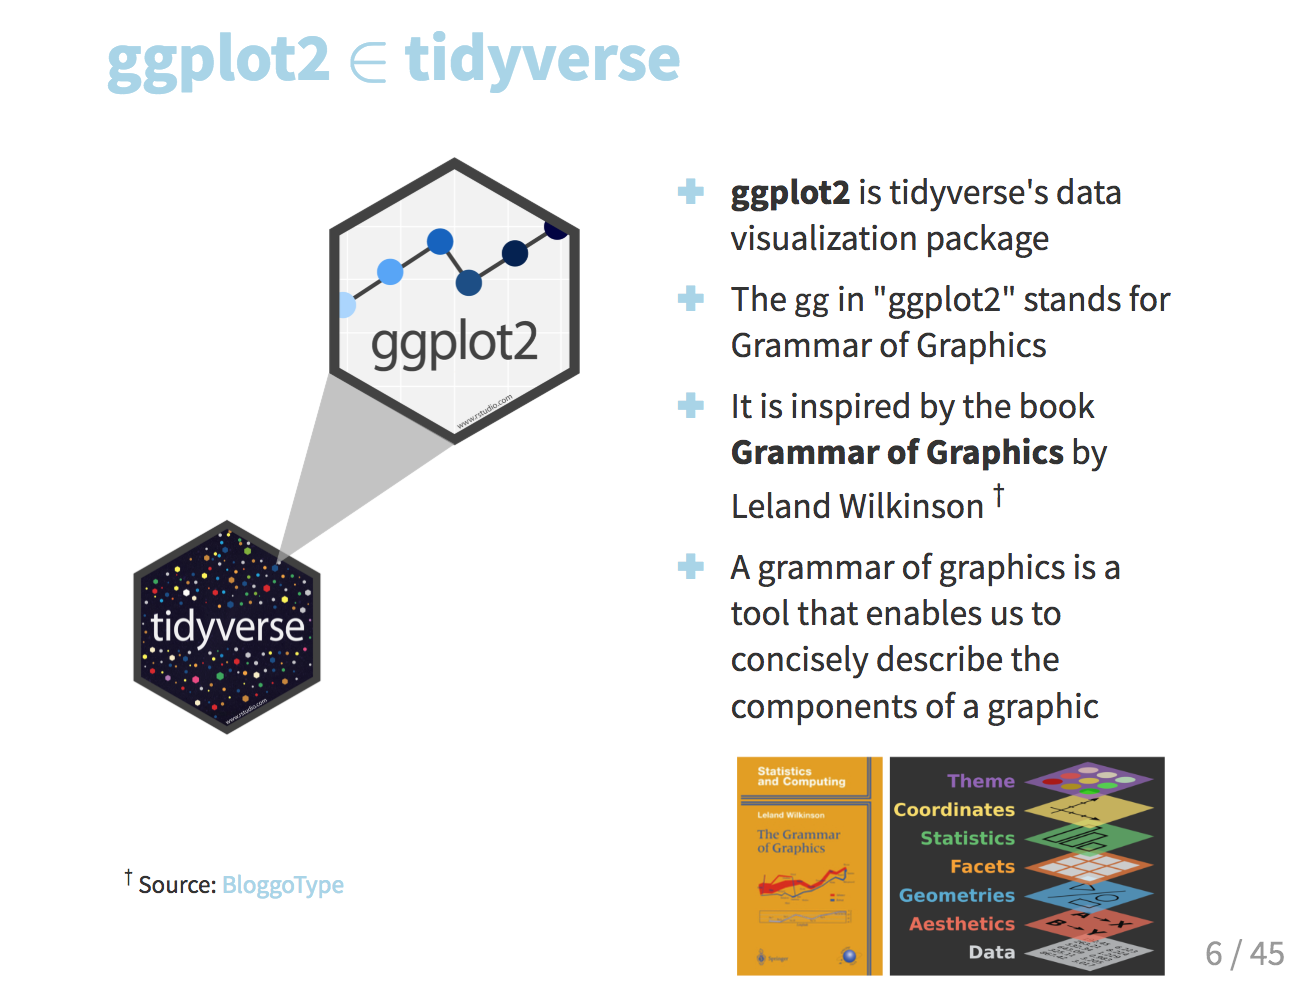
\includegraphics[width = 0.95\textwidth]{figures/visuals}
\end{center}

\vfill

\end{frame}

% -------------------------------------------------------------------

\begin{frame}
\frametitle{Use clear and consistent formatting}

\begin{center}
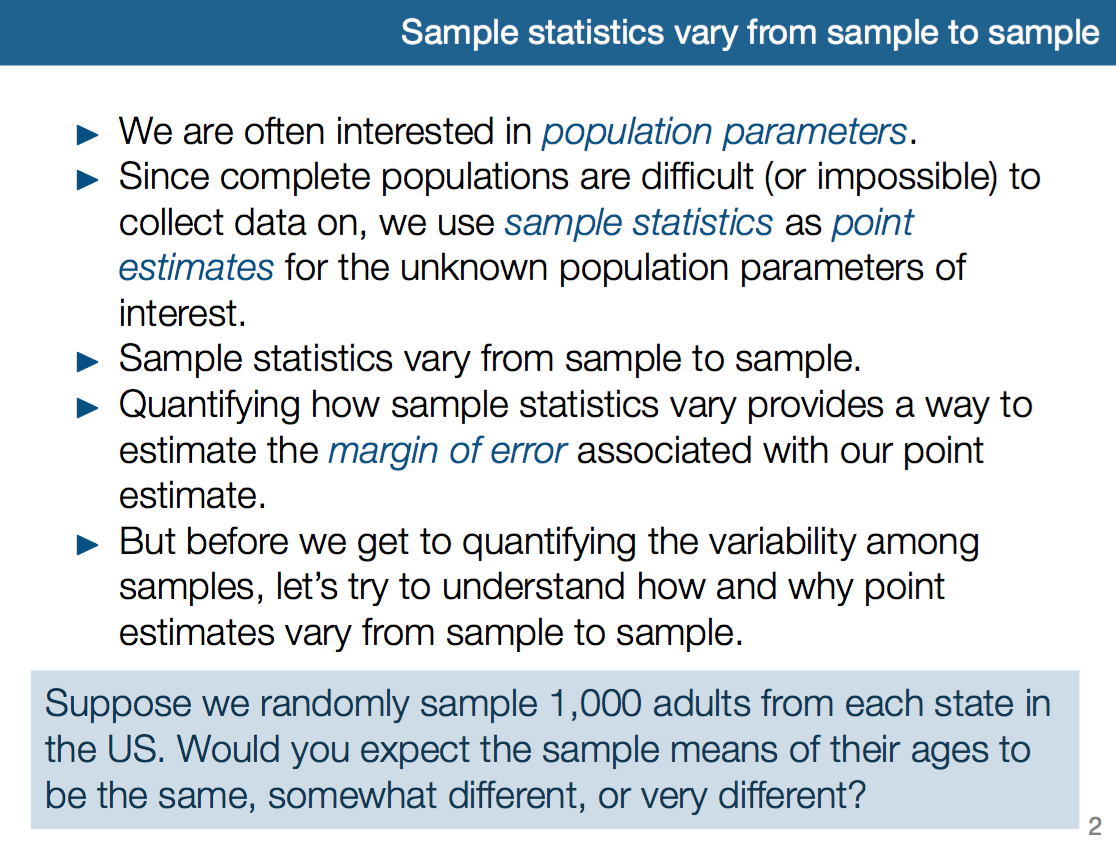
\includegraphics[width = 0.95\textwidth]{figures/disc-question}
\end{center}

\vfill

\end{frame}

% -------------------------------------------------------------------

\begin{frame}
\frametitle{Highlight main messages}

\begin{center}
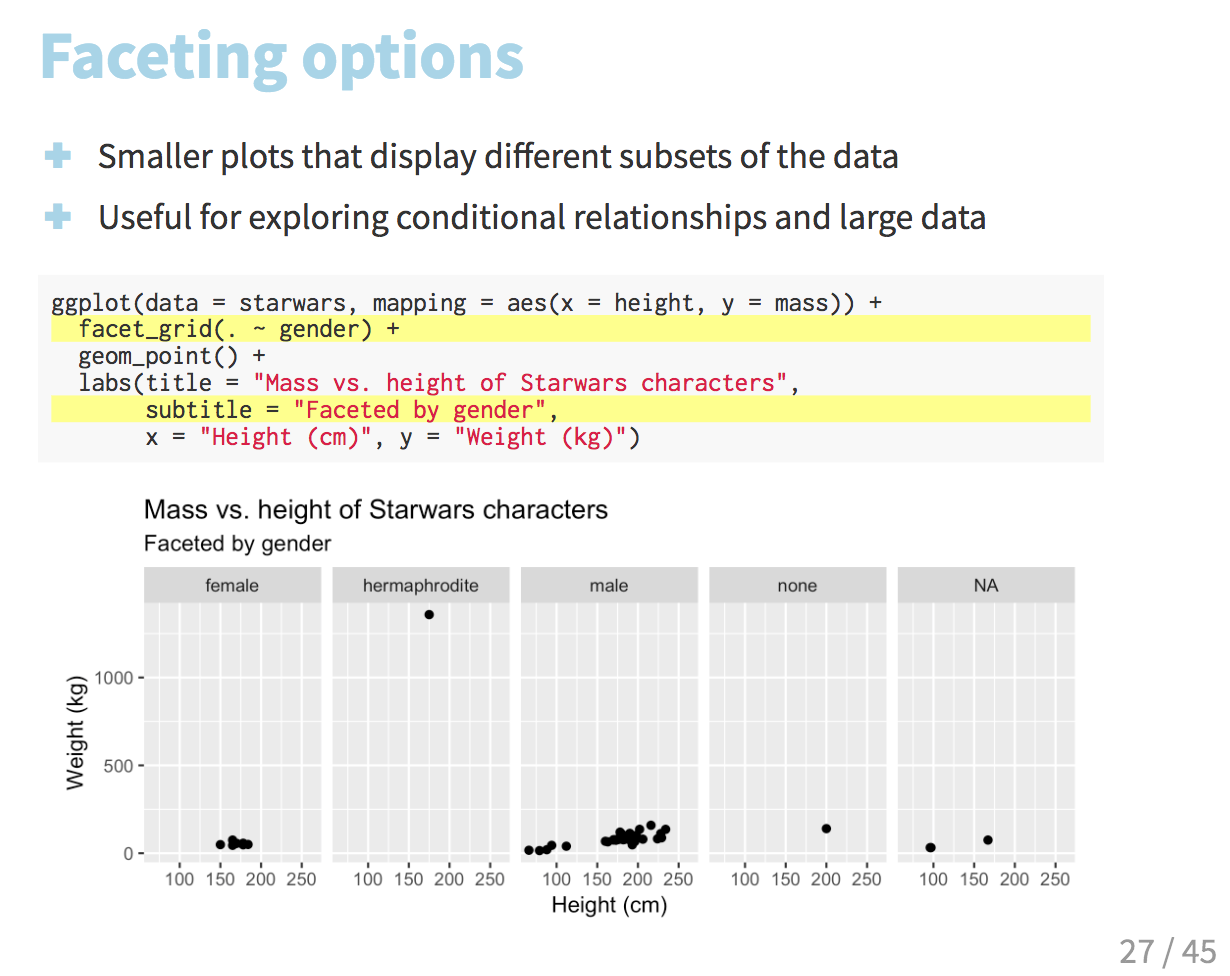
\includegraphics[width = 0.95\textwidth]{figures/highlighting}
\end{center}

\vfill

\end{frame}

% -------------------------------------------------------------------

\begin{frame}[fragile]
\frametitle{Hide the answers}

\begin{itemize}

\item If using LaTeX / Beamer, this is easy:

\begin{itemize}

\item For slides you show in class:

\begin{verbatim}
\newcommand{\soln}[1]{\textit{#1}}
\end{verbatim}

\soln{I'm on the slides shown in class, but not on the posted slides.}

\item For slides posted for students:

\begin{verbatim}
\newcommand{\soln}[1]{}
\end{verbatim}

\end{itemize}

\pause

\item Possible to achieve similar formatting with R Markdown as well

\pause

\item For Keynote, PowerPoint etc. you might need to manually add/remove text

\end{itemize}


\end{frame}

% -------------------------------------------------------------------

\begin{frame}
\frametitle{Make it a little less "traditional"}

\begin{center}
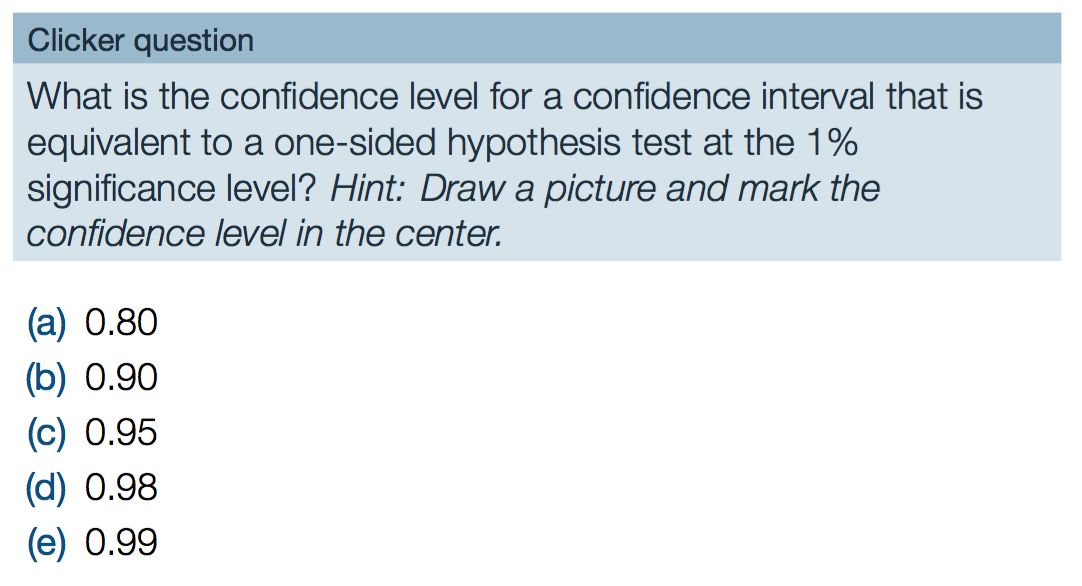
\includegraphics[width = 0.95\textwidth]{figures/clicker-question}
\end{center}

\vfill

\end{frame}

% -------------------------------------------------------------------

\begin{frame}
\frametitle{Classroom response systems}

\begin{itemize}

\item Clickers are one good option
\begin{itemize}
\item Pro: No distraction, can use for "closed book" assessments, can be used to track participation
\item Con: "Unitasker", expensive
\end{itemize}

\pause

\item Another option is an online polling system, e.g. PollEverywhere \href{https://pollev.com/minecetinkay621}{\textcolor{orange}{\texttt{[DEMO]}}}

\pause

\item Think about how they factor into overall assessment (anything <5\% of grade does not get sufficient student attention)

\end{itemize}

\end{frame}

% -------------------------------------------------------------------

\section{Flipped classroom}

% -------------------------------------------------------------------

\begin{frame}
\frametitle{Flipped classroom definition}

\begin{itemize}

\item The flipped classroom is a pedagogical model in which the typical lecture and homework elements of a course are reversed. 

\pause

\item Short video lectures are viewed by students at home before the class session, while in-class time is devoted to exercises, projects, or discussions.

\end{itemize}

\end{frame}

% -------------------------------------------------------------------

\section{Team-based learning (TBL)}

% -------------------------------------------------------------------

\begin{frame}
\frametitle{TBL Definition}

Team-Based Learning is an evidence based collaborative learning teaching strategy 
designed around units of instruction, known as ``modules," that are taught in a three-step cycle: 

\begin{enumerate}
\item preparation
\item in-class readiness assessment
\item application exercises
\end{enumerate}

\begin{center}
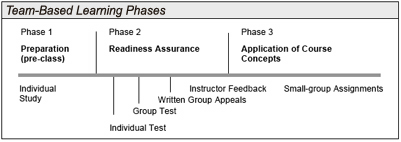
\includegraphics[width = 0.8\textwidth]{figures/TBLPhases}
\end{center}

\end{frame}

% -------------------------------------------------------------------

\begin{frame}
\frametitle{Preparing students for the preparation stage}

\begin{itemize}

\item List of clear learning objectives for the module

\item Textbook reading and/or videos

\item Practice questions

\end{itemize}

\end{frame}

% -------------------------------------------------------------------

\begin{frame}
\frametitle{Readiness assessment}

\begin{itemize}

\item Individual, and then as a Team

\item Delivered via a method that allows the instructor to quickly view results to determine which questions to review

\item Questions should be very clearly tied to learning objectives

\item Good RA design: Average student who studied can get a roughly 80\% individually, and 100\% as a team

\end{itemize}

\end{frame}

% -------------------------------------------------------------------

\begin{frame}
\frametitle{Application exercises}

\begin{center}
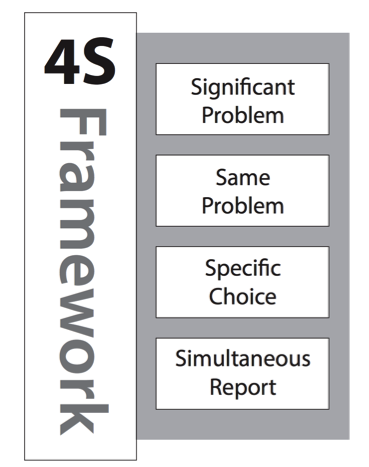
\includegraphics[width = 0.4\textwidth]{figures/4s}
\end{center}

\end{frame}

% -------------------------------------------------------------------

\begin{frame}
\frametitle{Teams}

\alert{What are your thoughts on the following aspects of team creation? What are pros and cons that you can think of for each option?}

\begin{itemize}

\item Formation: Student choice vs. assigned

\item Consistency: Same team throughout the semester vs. changing

\item Makeup: Homogenous vs. heterogenous with respect to background in course material

\end{itemize}

\end{frame}

% -------------------------------------------------------------------

\begin{frame}
\frametitle{Challenges for large clases}

\begin{itemize}

\item Need for additional instructor / TA bodies in the class

\pause

\item Timing of active components

\pause

\item ``Simultaneous reveal" of application exercises

\pause

\item Managing team dynamics

\end{itemize}

\end{frame}

% -------------------------------------------------------------------


\begin{frame}
\frametitle{Team based learning}

\vfill

\alert{
What are advantages / disadvantages for using team based learning pedagogy in your class?
}

\vfill

\end{frame}

% -------------------------------------------------------------------

\section{Hybrid models}

% -------------------------------------------------------------------

\begin{frame}
\frametitle{Hybrid models}

\begin{itemize}

\item Don't feel like you have to limit yourself to the strict definition of a specific pedagogy

\pause

\item Think about how you can borrow ideas from various pedagogies to make the most of your course

\end{itemize}

\end{frame}


% -------------------------------------------------------------------

\begin{frame}{Ex: Sta 101 - Intro Stats}
\frametitle{}

\begin{itemize}

\item Course is divided into seven learning units. 

\pause

\item Each unit has a set of learning objectives and required and suggested readings, videos, etc. Students are expected to watch the videos and/or complete the readings and familiarize themselves with the learning objectives. 

\pause

\item Begin the unit with a readiness assessment: 10 multiple choice questions that you answer using clickers and then re-take in teams using scratch off sheets.

\pause

\item Rest of the class split between discussion of the material and application exercises completed in teams. All class materials posted on course website.

\pause

\item Within each unit complement learning with problem sets and labs.

\pause

\item Wrap up each unit with a performance assessment.

\end{itemize}

\end{frame}

% -------------------------------------------------------------------

\section{Regardless of pedagogy}

% -------------------------------------------------------------------

\begin{frame}
\frametitle{Regardless of pedagogy...}

... you should have a

\begin{itemize}

\item detailed syllabus that clearly outlines all expectations and course logistics

\item a well organized course website (better -- for you -- if some components are public!) 

\end{itemize}

\end{frame}

% -------------------------------------------------------------------

\section{Visit a class}

% -------------------------------------------------------------------

\begin{frame}
\frametitle{Visit a class}

\begin{itemize}

\item Visit one (or more) classes (not lab session) between now and November 6

\item You're welcomed to visit my class: STA 112FS - TuTh 10:05 - 11:20 at Link Classroom 1

\item Reach out to any other faculty member to ask for their permission for a visit and whether there is a particular day they prefer you attend

\end{itemize}

\end{frame}

% -------------------------------------------------------------------




\end{document}